\chapter{Propriétés générales des détecteurs}
Un \textbf{détecteur} est un instrument qui mesure une des grandeurs qui caractérisent une particule.
Ici, on considèrera uniquement les particules provenant (in)directement des phénomènes nucléaires 
pour limiter le domaine des énergies. Un détecteur "faisant" tout (dit \textit{universel}) n'existe 
pas et il faudra concevoir différent types de détecteurs selon les besoins.\\

Il existe principalement trois types de mesures 
\begin{description}
\item[Moniteur] Détecteur pour des mesures immédiates de doses
\footnote{Energie déposée par unité de masse.} 
(chambre d'ionisation, "dosimètre", \dots )
\item[Dosimètre] Détecteur pour des mesures de dose intégrées sur
une période (film)
\item[Spectromètre]Détecteur pour l'identification des particules
indicentes
\end{description}

\section{Principes de base de la détection}%sl6
Tous les détecteurs sont basés sur le même principe fondamental : 
transférer la totalité (ou une partie) de l'énergie de la particule
incidente dans le détecteur ou elle est convertie dans une autre
forme, analysable et quantifiable. \\

	\begin{wrapfigure}[8]{r}{4cm}
	\vspace{-5mm}
	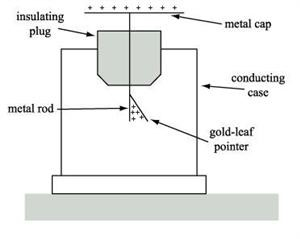
\includegraphics[scale=0.5]{ch7/image1}
	\captionof{figure}{ }
	\end{wrapfigure}
Historiquement, le premier appareil de métrologie nucléaire était 
l'\textit{électroscope}. Une tige métallique le constituant 
(chargée positivement) et placé près d'une feuille d'or. A cause de 
la répulsion entre les charges positives, la tige s'écartait de 
sa position d'équilibre. Lorsqu'une particule ionise l'air, il y
a un retour à l'équilibre à cause de la production de paires de
charges positives et négatives dans l'enceinte. Les charges
négatives vont en effet migrer vers la tige et la feuille, 
diminuant la quantité de charge positive : l'angle de déviation 
diminue.\\

Un électroscope est donc sensible à la quantité totale $N_i$ de
charges négatives et positives $Q$ produites dans l'enceinte
\begin{equation}
N_i=\frac{E_{abs}}{W}
\end{equation}
Les détecteurs modernes se basent sur le même principe. On mesure
toujours le nombre de rayonnements via la formation d'une impulsion
électrique. On comprend ici l'importance de $W$ car plus on a de 
charges, meilleur est la résolution. Choisir un matériau de 
détection, c'est choisir $W$.\\

Ainsi, toute les méthodes de détection sont basées sur la détection
des particules chargées (mesure \textit{directe}) tandis que les particules
neutres doivent interagir et produire des particules chargées 
avant de pouvoir être détectée (mesure \textit{indirecte}). Il 
existe trois principales méthodes de détection
\begin{enumerate}
\item Détecteur à gaz
\item Détecteurs à semiconducteurs
\item Scintillateurs
\end{enumerate}

\section{Modèle simplifié de détecteur}%sl9
Considérons  un détecteur hypothétique soumis à l'interaction d'une
particule chargée ou non dans son volume actif via l'un des
mécanismes discutés dans la partie précédente. On suppose que le 
temps d'interaction est court, l'énergie est donc déposée 
\textbf{instantanément}. Il y a dès lors apparition de $Q$ dans le
volume actif du détecteur en $t=0$. La collection de cette charge 
forme le signale électrique de base et la collection de celle-ci 
se fait via l'imposition d'un champ électrique faisant migrer les
charges dans des directions opposées avant d'être collectée.\\

Le temps de collection de charge $t_c$ dépend du type de détecteur
(mobilité des charges en son sein, distance à parcourir,\dots) et
de ce qu'on veut en faire. La réponse du détecteur est donnée par
\begin{equation}
\int_0^{t_c} i(t) dt=Q
\end{equation}
L'amplitude et la durée de chaque impulsion de courant dépend du 
type d'interaction.\\

La probabilité d'observer les rayonnements est soumise à la 
statistique de \textsc{Poisson} tandis que le temps entre deux 
impulsion est lié à la distribution d'\textsc{Erlang}. Le problème
est que si deux particules déposent leurs énergies en même temps, 
le courant mesuré sera la somme des deux et on ne peut plus 
distinguer les deux particules. On supposera toujours que le 
\textbf{nombre moyen de désintégration par unité de temps } $a$ est
suffisamment "faible" pour que chaque particule individuelle donne
une seule impulsion.


\subsection{Modes de fonctionnement}%sl12
Il existe trois modes de fonctionnement pour un détecteur
\begin{enumerate}
\item \textit{Mode courant}. On l'utilise quand le taux 
d'événements est très élevé et quand superposition : ne permet donc
pas la spectroscopie
\item \textit{Mode fluctuation}. Utilise quand l'on a deux types 
de rayonnements différents à différencier,mais peu utilisé en 
pratique. 
\item \textit{Mode impulsion}. Le favori.
\end{enumerate}

	\subsubsection{Mode courant}%sl13
	Un ampèremètre est connecté au détecteur de sorte à mesurer le
	courant (de l'ordre du pA). Celui-ci va mesurer un courant qui
	sera la moyenne des courants enregistré suivant un temps $T$, 
	le temps de résolution de l'appareil
	\begin{equation}
	I(t)=\frac{1}{T}\int_{t-T}^t i(t')dt'
	\end{equation}
	On obtient donc un courant moyen $I_0$ tel que $I_0=rQ$ où 
	$r$ est le taux d'interaction et $Q$ la charge produite par 
	interaction
	\begin{equation}
	I_0=r\frac{E_{abs}}{W}e
	\end{equation}
	Cette méthode est utilisées lorsqu'il y a superposition.
	
	\subsubsection{Mode fluctuation}%sl14
	Ce mode porte parfois le nom de son inventeur, 
	\textsc{Campbell}, en \textit{1914}. On bloque un courant 
	moyen $I_0$ et seulement les fluctuations $\sigma_I(t)$ sont
	mesurées
	\begin{equation}
	\overline{\sigma_I^2(t)}=\frac{1}{T}\int_{t-T}^t[I(t')-
	I_0]^2dt'=\frac{1}{T}\int_{t-T}^t\sigma_i^2(t')dt'
	\end{equation}		
	Comme nous avons uns statistique de \textsc{Poisson} (où $n$ 
	est le nombre d'événements enregistrés pendant un temps $T$), 
	on sait que
	\begin{equation}
	\sigma_n=\sqrt{n}=\sqrt{rT}
	\end{equation}
	Si chaque impulsion correspond à la même charge $Q$
	\begin{equation}
	\frac{\overline{\sigma_I(t)}}{I_0}=\frac{\sigma_n}{n}=\frac{1}
	{\sqrt{rT}}
	\end{equation}
	Comme par définition $I_0=rQ$, nous avons
	\begin{equation}
	\overline{\sigma_I^2(t)}=\frac{rQ^2}{T}
	\end{equation}
	En pratique on bloque le courant moyen, on mesure les 
	fluctuations, on met le résultat au carré et on sait que la 
	réponse est proportionnelle à $r$ et $Q^2$. Grâce à ce 
	$Q^2$, certains rayonnements (dans le cas ou plusieurs 
	rayonnements différents sont présents) auront une pondération
	plus forte. Il sera dès lors possible de les discriminer. En 
	pratique ceci n'est jamais utilisé car il existe d'autre 
	techniques plus simples.
	
	\subsubsection{Mode impulsion}%sl17
	Le détecteur est ici conçu pour enregistrer individuellement
	chaque rayonnement interagissant dans son volume actif. Le 
	signal impulsionnel dépendra des caractéristiques d'entrée du 
	circuit auquel le détecteur est connecté ($R,C,V(t)$).\\

	\begin{wrapfigure}[11]{r}{4cm}
	\vspace{-5mm}
	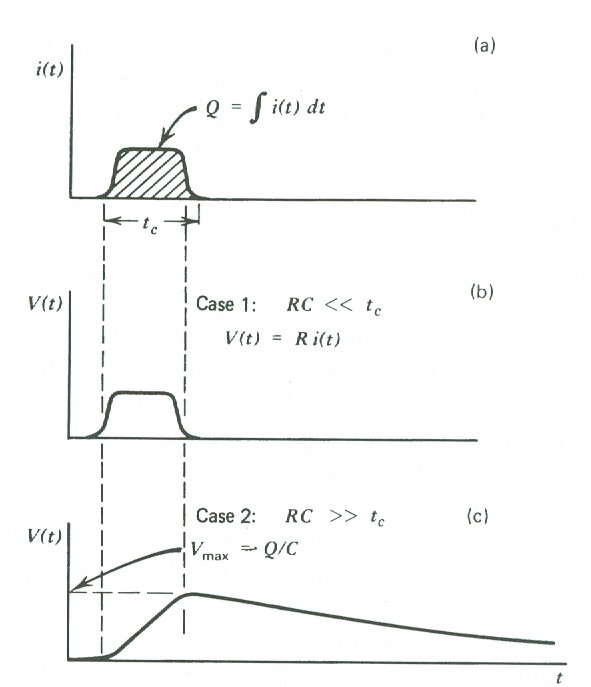
\includegraphics[scale=0.25]{ch7/image2}
	\captionof{figure}{ }
	\end{wrapfigure}

	Il existe deux fonctionnements "extrêmes" en fonction de la
	valeur de $\tau =RC$.
	\begin{enumerate}
	\item $\tau\ll t_c$. Il s'agit du deuxième graphique. 
	L'information recueillie est très précise niveau temps, mais 
	pas du tout en amplitude : on l'utilise pour des taux de 
	comptage élevés ou lorsque la dimension temporelle est plus
	importante que l'énergétique.
	\item $\tau \gg t_c$. Il s'agit du dernier graphique où l'on 
	voit que la croissance/décroissance se fait très lentement. 
	Cette fois-ci le maximum en amplitude est facilement 
	distinguable mais il ne faut pas qu'une deuxième impulsion ai
	lieu sans être revenu à zéro. Il s'agit du mode le plus 
	commun pour peu que les impulsions ne soient pas trop 
	rapprochées dans le temps.
	\end{enumerate}\ 
	
	Il s'agit du mode le plus utilisé car il possède une bien 
	meilleure sensibilité que les deux autres (on peut distinguer
	chaque impulsion individuellement) mais aussi parce que chaque
	impulsion apporte une information (le calcul d'un courant 
	moyen implique une perte d'informations).
	
\section{Spectrométrie des rayonnements}%sl20	
Pour se faire, il faut d'abord être en mode impulsion ($\tau\gg
t_c$) et avoir de grands nombres d'impulsions. Celles-ci diffèrent
en amplitude car chaque interaction n'implique par l'absorption 
totale de l'énergie de la particule incidente mais aussi à cause
de la réponse inhérente du détecteur qui ne fourni pas un signal
constant pour une énergie donnée.\\

La distribution des amplitudes des impulsions est une propriété
\textbf{fondamentale} du signal de sortie. Il convient de 
l'utiliser correctement pour obtenir des informations sur le 
rayonnement incident et ainsi faire de la \textbf{spectrométrie
des rayonnements}.\\

On utilise généralement la méthode de la \textit{distribution 
différentielles des hauteurs d'impulsions}

	\begin{wrapfigure}[8]{r}{5.4cm}
	%\vspace{-3mm}
	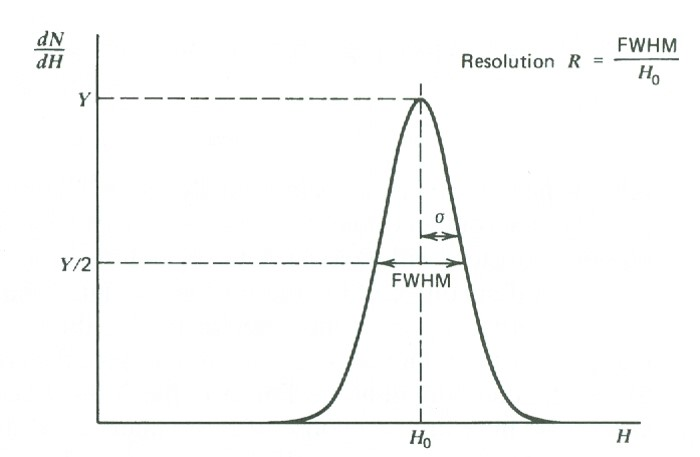
\includegraphics[scale=0.3]{ch7/image3}
	\captionof{figure}{ }
	\end{wrapfigure}\ 
 
 
\begin{itemize}
\item[$\bullet$] L'abscisse est une échelle linéaire des amplitudes
en impulsion
\item[$\bullet$] On mesure $dN/dH$ que l'on place en ordonnée. 
$dN$ est le nombre différentiel d'impulsions observées avec une
amplitude qui correspond à l'incrément différentiel $dH$. Le 
rapport des deux donne donc la largeur du canal : un graphique en 
colonne délimitée par un min et un max et on compte les 
impulsions entre ces deux bornes. 
\item[$\bullet$] On intègre : le nombre d'impulsions pour lesquels
l'amplitude se situe entre 2 valeurs spécifiques est obtenue par
intégration de la surface entre ces 2 limites.
\item[$\bullet$] Souvent des pics $H_0$ ont une énergie précises 
qui indique la détection d'une particule incidente caractérisé par
une énergie précise.
\item[$\bullet$] Souvent linéaire en pratique : $H_0 = KN_i$.
\end{itemize}\ 

La résolution en énergie $R$ du détecteur est par convention 
définie comme la largeur à mi-hauteur du pic divisée par la 
position du maximum. Une bonne résolution, correspond donc à une
petite valeur de $R$.

\subsection{Résolution du détecteur}%sl23
A cause du grand nombre de processus impliqués, cette détermination
est complexe. Si le nombre d'ionisation suit une loi de 
\textsc{Poisson}, on sait que $\sigma(H_0)=K\sqrt{N_i}$. Sachant
que $FWHM = 2\sqrt{2\ln 2}\sigma$, la résolution vaut
\begin{equation}
R=\frac{\mbox{FWHM}}{H_0}=\frac{2.35\sigma}{H_0}=\frac{2.35K\sqrt{N_i}}{KN_i}=\frac{2.35}{\sqrt{N_i}}=2.35\sqrt{\frac{W}{E_{abs}}}
\end{equation}
La résolution s'améliore (diminution de $R$) lorsque $N_i$ 
augmente, c'est-à-dire lorsque $W$ diminue. De façon générale, 
nous avons
\begin{equation}
R_{SC} < R_{gaz} < R_{Scintillateur}
\end{equation}
On peut également introduire le facteur empirique de \textsc{Fano}
$F$  (incluant les différences par rapport à la loi de 
\textsc{Poisson}) $\sigma_i^2 = FN_i$ pour ré-écrire la 
résolution comme
\begin{equation}
R=2.35\frac{\sqrt{FN_i}}{N_i}=2.35\sqrt{\frac{FW}{E_{abs}}}
\end{equation}
Pour beaucoup de détecteurs (SC, gaz), $F<1$.


\section{Efficacité de détection}%sl26
Que ce soit pour des particules chargées ayant une interaction 
directe ou non-chargées présentant une interaction indirecte, il 
y a nécessite d'introduire la notion d'efficacité qui selon 
deux classe : \textbf{absolue} et \textbf{intrinsèque}.
\begin{enumerate}
\item \textit{Efficacité absolue}. Dépend des propriétés du 
détecteur et de la géométrie de détection
\begin{equation}
\epsilon_{abs}=\frac{\mbox{nombre d'impulsions enregistr\'ees}
}{\mbox{nombre de rayonnements \'emis par la source}}
\end{equation}
\item \textit{Efficacité intrinsèque}. Dépend des propriétés du
détecteur.
\begin{equation}
\epsilon_{int}=\frac{\mbox{nombre d'impulsions enregistr\'ees}
}{\mbox{nombre de rayonnements incidents sur le d\'etecteur}}
\end{equation}
Pour une source isotrope, $\epsilon_{int}=\epsilon_{abs} (4\pi/
\Omega)$ où $\Omega$est l'angle solide du détecteur vu de la 
position de la source.
\end{enumerate}\ 

Il est également possible de définir l'efficacité en fonction de 
la nature de l'événement enregistré. Si on ne discrimine aucune
impulsion, on parle d'\textit{efficacité totale}  $\epsilon_{tot}$.
Si on considère que les impulsion qui ont déposées toute leur 
énergie on parle d'\textit{efficacité de pic} $\epsilon_{peak}$.\\

On utilise souvent (combinaison des deux précédents) l'\textit{
efficacité intrinsèque de pic} $\epsilon_{ip}$ qui est la 
valeur la plus souvent tabulée. Pour une source de photons isotrope
et monoénergétique émettant $S$ rayonnements pendant un temps $T$
et $N_p$, le nombre d'événements correspondant au pic d'absorption
totale enregistrés pendant le temps $T$
\begin{equation}
S=N_p\frac{4\pi}{\epsilon_{ip}\Omega}
\end{equation}\ \\


Rappelons que l'angle solide est définie par $\Omega=\int_A
\frac{\cos\theta}{r^2}dA$ et que dès lors, pour la source 
positionnée sur l'axe d'un cylindre représentant le détecteur
\begin{equation}
\Omega=2\pi\left( 1-\frac{r}{\sqrt{r^2+d^2}}\right)
\end{equation}
Ce qui donne $\Omega\simeq \frac{\pi d^2}{r^2}$ pour $r\gg d$.



\section{Temps mort}%sl31
Le temps mort est le temps minimum qui doit séparer deux événements
pour être enregistrés comme deux impulsions distinctes. Il existe
deux modèles de temps mort\footnote{Les systèmes réels sont 
intermédiaires}
\begin{enumerate}
\item \textit{Paralysable} (ou \textit{cumulatif})
\item \textit{Non-paralysable} (ou \textit{non-cumulatif})
\end{enumerate}

\subsection{Modèle non-paralysable}
Soit $m$ le taux d'interaction réel, $m$ le taux d'interaction 
enregistré et $\tau$ le temps mort. Ce modèle stipule que la 
fraction de temps pendant lequel le détecteur est mort vaut
$m\tau$. Le taux auquel les événements sont perdus est donc 
$nm\tau$. Comme le taux peut également s'écrire $n-m$, en 
égalant les deux on trouve
\begin{equation}
n=\frac{m}{1-m\tau}\qquad\Leftrightarrow\qquad 
m=\frac{n}{1+n\tau}
\end{equation}

\subsection{Modèle paralysable}
Ici les périodes de temps mort n'ont pas une longueur fixe. La
distribution des intervalles entre deux événements est donné par
\begin{equation}
P(t)dt=n\exp{(-nt)}dt
\end{equation}
La probabilité que $t>\tau$ vaut alors
\begin{equation}
P(t>\tau)=n\int_\tau^\infty \exp{(-nt)}dt=\exp{(-n\tau)}
\end{equation}
Le taux d'occurrence de ces intervalles est obtenu en 
multipliant cette expression par le taux réel $n$
\begin{equation}
m=n\exp{(-n\tau)}
\end{equation}



\begin{center}
	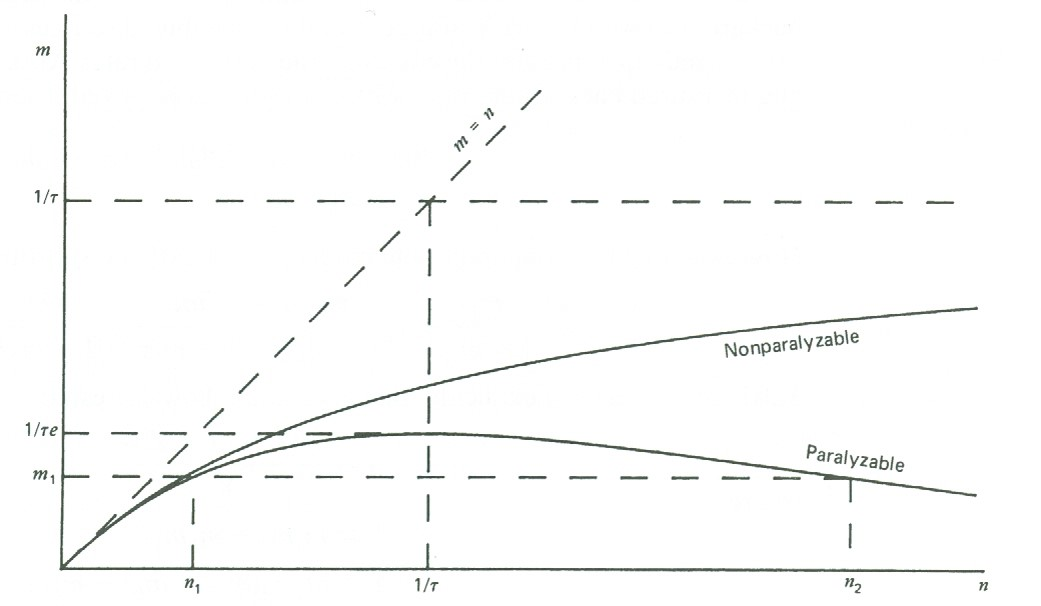
\includegraphics[scale=0.5]{ch7/image4}
	\captionof{figure}{Variation de $m$ en fonction de $n$. 
	Pour $n$ faible, $m \approx n(1-n\tau)$. Pour les grandes
	valeurs de $N$ on ne considère plus des impulsions mais un 
	courant ce qui règle le problème.}
\end{center}



























